\documentclass[a4paper]{article}
\usepackage[utf8]{vietnam}
\usepackage{attachfile} 
\usepackage{amsmath}  % ghi cac phep toan
%\usepackage{indentfirst}  % auto intended - tự thụt đầu dòng
\usepackage{a4wide,amssymb,epsfig,latexsym,array,hhline,fancyhdr}
\usepackage{caption,subcaption} % chú thích
\usepackage{graphicx}     % chèn hình ảnh
\usepackage{listings}       % chèn code c, cpp, python, .. vào
\usepackage{hyperref}     % tele to other tittle
\usepackage{parskip}      % space between line

\definecolor{codegreen}{rgb}{0,0.6,0}
\definecolor{codegray}{rgb}{0.5,0.5,0.5}
\definecolor{codepurple}{rgb}{0.58,0,0.82}
\definecolor{backcolour}{rgb}{0.95,0.95,0.92}
\lstdefinestyle{mystyle}{
    backgroundcolor=\color{backcolour},   
    commentstyle=\color{codegreen},
    keywordstyle=\color{magenta},
    numberstyle=\tiny\color{codegray},
    stringstyle=\color{codepurple},
    basicstyle=\ttfamily\footnotesize,
    breakatwhitespace=false,         
    breaklines=true,                 
    captionpos=b,                    
    keepspaces=true,                 
    numbers=left,                    
    numbersep=5pt,                  
    showspaces=false,                
    showstringspaces=false,
    showtabs=false,                  
    tabsize=2
}
\lstset{style=mystyle}
\definecolor{light-gray}{gray}{0.95}
\newcommand{\code}[1]{\colorbox{light-gray}{\texttt{#1}}}
\usepackage[framemethod=tikz]{mdframed}% For highlighting paragraph backgrounds


\usepackage{lastpage}    % đánh số trang
\usepackage[a4paper, top=2cm, bottom=4cm, left=2.5cm, right=2.5cm]{geometry}

%=======================================================
\setlength{\headheight}{40pt}
\pagestyle{fancy}
\fancyhead{}
\fancyhead[L]{
 \begin{tabular}{rl}
    \begin{picture}(25,15)(0,0)
    \put(0,-8){
\includegraphics[width=8mm, height=8mm]{images/hcmut.png}}
   \end{picture}&
	\begin{tabular}{l}
		\textbf{\bf \ttfamily Trường Đại Học Bách Khoa Tp.Hồ Chí Minh}\\
		\textbf{\bf \ttfamily Khoa Khoa Học \& Kỹ Thuật Máy Tính}
	\end{tabular} 	
 \end{tabular}
}
\fancyhead[R]{
	\begin{tabular}{l}
		\tiny \bf \\
		\tiny \bf 
	\end{tabular}  }
\fancyfoot{} % clear all footer fields
\fancyfoot[L]{\scriptsize \ttfamily Đại số tuyến tính - CSLT - 242}
\fancyfoot[R]{\scriptsize \ttfamily Page {\thepage}/\pageref{LastPage}}
\renewcommand{\headrulewidth}{0.5pt}
\renewcommand{\footrulewidth}{0.5pt}

\setcounter{secnumdepth}{3}
\setcounter{tocdepth}{3}
\makeatletter
\newcounter {subsubsubsection}[subsubsection]
\renewcommand\thesubsubsubsection{\thesubsubsection .\@alph\c@subsubsubsection}

\newcommand*\l@subsubsubsection{\@dottedtocline{3}{10.0em}{4.1em}}
\newcommand*{\subsubsubsectionmark}[1]{}
\makeatother


%\everymath{\color{blue}}%make in-line maths symbols blue to read/check easily
%=======================================================

%======================================================
\begin{document}
\begin{titlepage}
    \centering
    \textbf{\Large ĐẠI HỌC QUỐC GIA THÀNH PHỐ HỒ CHÍ MINH} \\
    \vspace{0.5cm}
    \textbf{\Large TRƯỜNG ĐẠI HỌC BÁCH KHOA} \\
    \textbf{\Large KHOA KHOA HỌC \& KỸ THUẬT MÁY TÍNH} \\
    \vspace{1.0cm}
    
\includegraphics[width=4.5cm]{images/hcmut.png} \\
    \vspace{0.8cm}
    \rule{\linewidth}{0.5mm} \\
    \vspace{0.3cm}
    {

    \LARGE\text{\textbf{BÁO CÁO BÀI TẬP LỚN}}\\
    \LARGE\text{\textbf{ĐẠI SỐ TUYẾN TÍNH}}\\
    \vspace{0.3cm}
    \huge \text{\textbf{Đề tài 10}}\\
    \vspace{0.15cm}
    \Large \text{\textbf{Phân tích Randomized SVD (Truncated SVD)}}\\
    \Large \text{\textbf{và ứng dụng trong nén dữ liệu}}\\
    \Large \text{\textbf{theo tỉ lệ năng lượng cho trước}}\\

    \vspace{0.4cm}
    \rule{\linewidth}{0.5mm}
    \vspace{0.4cm}

    \Large\text{Giảng viên hướng dẫn: Nguyễn Hữu Hiệp}\\
    \vspace{0.2cm}
    \Large\text{Nhóm L05 -- Danh sách thành viên}\\
    \vspace{0.15cm}
    \normalsize
    \begin{tabular}{rl}
        2213539 & Phạm Quốc Toàn \\
        2213496 & Nguyễn Quốc Tín \\
        2213299 & Nguyễn Trường Thịnh \\
        2213289 & Nguyễn Hữu Thịnh \\
        2213228 & Hồ Viết Thiên \\
        2213120 & Trương Hữu Thái \\
        2213080 & Trương Hồng Tấn \\
        2213063 & Nguyễn Trung Tân \\
        2212922 & Nguyễn Quang Sáng \\
    \end{tabular}\\
    \vspace{0.8cm}
    {\Large Thành phố Hồ Chí Minh, tháng 5/2026}}

\end{titlepage}
%======================================================


\newpage
\renewcommand{\contentsname}{Content}
\renewcommand{\figurename}{Figure}
\renewcommand{\tablename}{Table}

\tableofcontents
% =====================================================================
%   NỘI DUNG BÁO CÁO  -  ĐỀ TÀI 10
%   Phân tích Randomized SVD và ứng dụng nén dữ liệu theo tỉ lệ năng lượng
% =====================================================================

\newpage
% =====================================================================
\section{Mở đầu}
% =====================================================================

\subsection{Lý do chọn đề tài}

Trong kỷ nguyên dữ liệu lớn, kích thước các ma trận biểu diễn dữ liệu thực tế
(ảnh số, ma trận đánh giá, dữ liệu cảm biến, văn bản, \dots) thường vượt xa khả
năng lưu trữ và xử lý trực tiếp. Phân tích giá trị kỳ dị (Singular Value
Decomposition -- SVD) là một trong những công cụ trung tâm của đại số tuyến tính
hiện đại: nó cho phép tách một ma trận bất kỳ thành tích của ba ma trận có cấu
trúc đẹp, từ đó tạo ra cơ sở toán học cho hàng loạt ứng dụng như nén dữ liệu,
giảm chiều, khử nhiễu, hệ thống gợi ý và xử lý ảnh.

Tuy nhiên, thuật toán SVD cổ điển (thông qua phương pháp Golub--Kahan hay
Jacobi) có độ phức tạp $\mathcal{O}(mn\min(m,n))$ và đòi hỏi truy xuất toàn bộ
ma trận nhiều lần. Khi $m, n$ ở mức $10^5$ trở lên, cách tiếp cận này trở nên
bất khả thi cả về thời gian lẫn bộ nhớ. \textbf{Randomized SVD}, được Halko,
Martinsson và Tropp hệ thống hóa năm 2011, là một cách tiếp cận đột phá: dùng
phép chiếu ngẫu nhiên để rút trích nhanh một không gian con xấp xỉ tốt cho
$k$ giá trị kỳ dị lớn nhất, sau đó chỉ chạy SVD cổ điển trên một ma trận nhỏ
hơn nhiều. Phương pháp này có cơ sở toán học vững chắc, sai số kiểm soát được
và dễ song song hóa.

Đề tài tập trung vào Randomized SVD vì ba lý do:
\begin{itemize}
    \item \textbf{Tầm quan trọng toán học:} đây là một kết quả tiêu biểu của
    đại số tuyến tính số (numerical linear algebra) hiện đại, kết hợp xác suất,
    hình học và giải tích ma trận.
    \item \textbf{Lĩnh vực áp dụng rộng:} học máy, xử lý ảnh, hệ thống gợi ý,
    nén tín hiệu, phân tích văn bản (LSA), tin sinh học.
    \item \textbf{Vấn đề thực tế cụ thể:} bài toán giảm dung lượng lưu trữ và
    rút gọn chiều biểu diễn cho dữ liệu lớn, sao cho vẫn giữ được một tỉ lệ
    năng lượng (thông tin) $\eta$ cho trước.
\end{itemize}

\subsection{Mục tiêu của đề tài}

Báo cáo hướng tới các kết quả cụ thể sau:
\begin{itemize}
    \item Trình bày được cơ sở lý thuyết của SVD đầy đủ, Compact SVD và
          Randomized SVD; nêu rõ ý nghĩa toán học của từng đại lượng.
    \item Xây dựng được tiêu chuẩn chọn $k$ theo tỉ lệ năng lượng
          $$ \frac{\sum_{i=1}^{k}\sigma_i^2}{\sum_{i=1}^{r}\sigma_i^2} \;\ge\; \eta,$$
          và phân tích ý nghĩa của tham số $\eta$.
    \item Cài đặt thuật toán Randomized SVD và áp dụng cho một ma trận dữ liệu
          thực tế có kích thước lớn (trên $10^5$ phần tử).
    \item Tái dựng ma trận xấp xỉ hạng thấp $A_k$, lưu trữ dưới dạng dữ liệu nén
          $(U_k, \Sigma_k, V_k)$ và đánh giá sai số xấp xỉ
          $\|A - A_k\|_F$ theo chuẩn Frobenius.
    \item Phân tích mối quan hệ giữa tỉ lệ năng lượng giữ lại, sai số xấp xỉ và
          dung lượng lưu trữ; rút ra điều kiện thực tế để Randomized SVD đạt
          hiệu quả nén tốt.
\end{itemize}

\subsection{Phạm vi nghiên cứu}

\begin{itemize}
    \item \textbf{Đối tượng nghiên cứu:} ma trận thực $A \in \mathbb{M}_{m\times n}(\mathbb{R})$
          với $m\cdot n \ge 10^5$. Trong báo cáo, ma trận thí nghiệm là ma trận
          xếp hạng người dùng -- phim của bộ MovieLens 25M
          ($162\,541 \times 59\,047$).
    \item \textbf{Cân bằng lý thuyết -- ứng dụng:} báo cáo trình bày đầy đủ cơ
          sở toán học (định lý phổ, định lý Eckart--Young, hệ quả về chuẩn
          Frobenius) và áp dụng vào thực nghiệm bằng Python.
    \item \textbf{Nội dung không xét đến:} phiên bản phân tán/GPU của
          Randomized SVD, các biến thể khối (block) phức tạp, và phân tích sai
          số xác suất chi tiết (chỉ trình bày định tính).
\end{itemize}


% =====================================================================
\section{Cơ sở lý thuyết}
% =====================================================================

\subsection{Một số khái niệm chuẩn bị}

\paragraph{Hệ trực chuẩn và ma trận trực giao.}
Hệ véc-tơ $\{u_1, \dots, u_k\} \subset \mathbb{R}^m$ được gọi là
\emph{trực chuẩn} nếu $u_i^T u_j = \delta_{ij}$ ($\delta_{ij}=1$ khi $i=j$ và
bằng $0$ trong trường hợp ngược lại). Ma trận $U \in \mathbb{R}^{m\times m}$ với các
cột tạo thành hệ trực chuẩn gọi là \emph{ma trận trực giao}; khi đó
$U^T U = UU^T = I$, suy ra $U^{-1} = U^T$.

\paragraph{Chuẩn Frobenius.}
Với $A \in \mathbb{R}^{m\times n}$, định nghĩa
\[
\|A\|_F \;=\; \sqrt{\sum_{i=1}^m\sum_{j=1}^n a_{ij}^2}
       \;=\; \sqrt{\operatorname{tr}(A^T A)}.
\]
Chuẩn Frobenius bất biến qua phép nhân với ma trận trực giao: với mọi
$Q$ trực giao thì $\|QA\|_F = \|A\|_F$ và $\|AQ\|_F = \|A\|_F$.

\paragraph{Hạng của ma trận.} Hạng $r = \operatorname{rank}(A)$ là số chiều của
không gian cột (cũng bằng không gian hàng). Luôn có $r \le \min(m,n)$.

\subsection{Định lý phân tích giá trị kỳ dị (SVD)}

\begin{mdframed}[backgroundcolor=black!5]
\textbf{Định lý 2.1 (SVD đầy đủ).}\
Với mọi $A \in \mathbb{R}^{m\times n}$ tồn tại các ma trận trực giao
$U \in \mathbb{R}^{m\times m}$, $V \in \mathbb{R}^{n\times n}$ và một ma trận đường chéo
suy rộng $\Sigma \in \mathbb{R}^{m\times n}$ sao cho
\[
A \;=\; U\,\Sigma\,V^T,
\qquad
\Sigma = \operatorname{diag}(\sigma_1, \sigma_2, \dots, \sigma_p),
\quad p = \min(m,n),
\]
với $\sigma_1 \ge \sigma_2 \ge \dots \ge \sigma_p \ge 0$.
\end{mdframed}

\textbf{Ý nghĩa.}
\begin{itemize}
    \item Các cột $u_i$ của $U$ -- \emph{véc-tơ kỳ dị trái} -- là cơ sở trực chuẩn của
          không gian cột mở rộng của $A$;
    \item các cột $v_i$ của $V$ -- \emph{véc-tơ kỳ dị phải} -- là cơ sở trực chuẩn của
          không gian hàng mở rộng;
    \item các số $\sigma_i$ -- \emph{giá trị kỳ dị} -- đo \emph{mức độ kéo dãn} của
          ánh xạ tuyến tính $x\mapsto Ax$ theo từng hướng chính.
\end{itemize}

\textbf{Liên hệ với phổ.}
Đặt $A = U\Sigma V^T$. Khi đó
\[
A^T A \;=\; V\,\Sigma^T\Sigma\,V^T,
\qquad
A A^T \;=\; U\,\Sigma\Sigma^T\,U^T.
\]
Do đó $\sigma_i^2$ là trị riêng của $A^TA$ (và của $AA^T$); $v_i$ là véc-tơ
riêng của $A^TA$; $u_i$ là véc-tơ riêng của $AA^T$. Đây là cơ sở để chứng minh
sự tồn tại của SVD: ta áp dụng định lý phổ cho ma trận đối xứng nửa xác định
dương $A^TA$.

\subsection{Compact SVD (Reduced SVD)}

Gọi $r = \operatorname{rank}(A)$. Vì $\sigma_{r+1} = \dots = \sigma_p = 0$, ta có
\[
A \;=\; \sum_{i=1}^{p} \sigma_i u_i v_i^T \;=\; \sum_{i=1}^{r}\sigma_i u_i v_i^T.
\]
Định nghĩa
\[
U_r = [u_1 \,|\, u_2 \,|\, \dots \,|\, u_r] \in \mathbb{R}^{m\times r},\
\Sigma_r = \operatorname{diag}(\sigma_1,\dots,\sigma_r) \in \mathbb{R}^{r\times r},\
V_r = [v_1 \,|\, \dots \,|\, v_r] \in \mathbb{R}^{n\times r},
\]
ta thu được
\[
\boxed{\;A \;=\; U_r\,\Sigma_r\,V_r^T\;}
\]
là \emph{Compact SVD}. So với SVD đầy đủ, nó chỉ giữ lại các thành phần thực sự
đóng góp vào $A$, loại bỏ các cột tương ứng với $\sigma_i=0$. Khi $r \ll \min(m,n)$
(ma trận hạng thấp), Compact SVD tiết kiệm rất nhiều bộ nhớ.

\subsection{Định lý Eckart--Young -- xấp xỉ hạng thấp tốt nhất}

\begin{mdframed}[backgroundcolor=black!5]
\textbf{Định lý 2.2 (Eckart--Young 1936).}\
Với $1 \le k \le r$ và $A_k = \sum_{i=1}^{k}\sigma_i u_i v_i^T$, ta có
\[
\min_{\operatorname{rank}(B)\le k} \|A-B\|_F \;=\; \|A - A_k\|_F
\;=\; \sqrt{\sum_{i=k+1}^{r}\sigma_i^2}.
\]
\end{mdframed}

Nói cách khác, $A_k$ -- tổng của $k$ thành phần kỳ dị lớn nhất -- là
\emph{xấp xỉ hạng-$k$ tốt nhất} của $A$ theo chuẩn Frobenius. Đây là cơ sở
trực tiếp cho mọi kỹ thuật nén dữ liệu dựa trên SVD: nếu chấp nhận sai số
$\varepsilon$ thì chỉ cần giữ đủ số $k$ giá trị kỳ dị sao cho
$\sum_{i>k}\sigma_i^2 \le \varepsilon^2$.

\subsection{Năng lượng dữ liệu và tiêu chuẩn chọn $k$}

\paragraph{Khái niệm năng lượng.}
Với SVD ta có
\[
\|A\|_F^2 \;=\; \sum_{i=1}^{r}\sigma_i^2.
\]
Đại lượng $\|A\|_F^2$ được gọi là \emph{tổng năng lượng} (total energy) của
ma trận dữ liệu; mỗi $\sigma_i^2$ là \emph{năng lượng} đóng góp bởi thành phần
kỳ dị thứ $i$. Trên thực nghiệm với dữ liệu thực, dãy $\sigma_i^2$ thường suy
giảm rất nhanh theo $i$ -- đây chính là lý do nén dữ liệu khả thi.

\paragraph{Tiêu chuẩn năng lượng.}
Cho ngưỡng $\eta \in (0,1)$ (ví dụ $0.90, 0.95, 0.99$). Ta chọn $k$ nhỏ nhất
thỏa mãn
\begin{equation}\label{eq:energy-criterion}
\frac{\sum_{i=1}^{k}\sigma_i^2}{\sum_{i=1}^{r}\sigma_i^2} \;\ge\; \eta.
\end{equation}
Khi đó, theo Eckart--Young,
\[
\frac{\|A-A_k\|_F^2}{\|A\|_F^2} \;=\; 1 - \frac{\sum_{i=1}^{k}\sigma_i^2}{\sum_{i=1}^{r}\sigma_i^2} \;\le\; 1-\eta,
\]
tức tỉ lệ sai số bình phương được khống chế bởi $1-\eta$. Ví dụ $\eta=0.95$
đảm bảo $\|A-A_k\|_F^2 \le 0.05\,\|A\|_F^2$.


% =====================================================================
\section{Thuật toán Randomized SVD}
% =====================================================================

\subsection{Ý tưởng và động cơ}

Với ma trận $A$ kích thước cực lớn, ta chỉ cần thông tin về \emph{không gian
con chính} (principal range) của $A$ -- nơi tập trung gần như toàn bộ năng
lượng. Halko, Martinsson, Tropp \cite{halko2011} đề xuất một cách hiệu quả:
dùng \emph{phép chiếu ngẫu nhiên} để rút ra không gian con này, rồi chỉ chạy
SVD đầy đủ trên một ma trận có kích thước rất nhỏ $(k+p)$.

Cụ thể, nếu $\Omega \in \mathbb{R}^{n\times(k+p)}$ là một ma trận chuẩn Gauss ngẫu
nhiên thì $Y = A\Omega$ \emph{với xác suất rất cao} chứa $k$ véc-tơ kỳ dị trái
quan trọng nhất của $A$ trong không gian cột của nó. Tham số $p$ (over-sampling,
thường $5$--$10$) tăng đáng kể độ ổn định của thuật toán.

\subsection{Thuật toán}

\begin{mdframed}[backgroundcolor=black!5]
\textbf{Thuật toán: Randomized SVD bậc} $k$.\\[2pt]
\textbf{Đầu vào:} ma trận $A \in \mathbb{R}^{m\times n}$, hạng mục tiêu $k$, over-sampling $p$
(mặc định $p=10$), số bước power iteration $q$ (mặc định $1$--$2$).\\
\textbf{Đầu ra:} $U_k \in \mathbb{R}^{m\times k}, \Sigma_k \in \mathbb{R}^{k\times k}, V_k \in \mathbb{R}^{n\times k}$.

\smallskip
\begin{enumerate}
    \item \textbf{Sinh ma trận chiếu ngẫu nhiên:} sinh ma trận
    $\Omega \in \mathbb{R}^{n\times(k+p)}$ với các phần tử i.i.d. $\mathcal{N}(0,1)$.
    \item \textbf{Lấy mẫu cột:} tính $Y = A\Omega \in \mathbb{R}^{m\times(k+p)}$.
    \item \textbf{Power iteration} (tùy chọn, tăng độ chính xác khi phổ
    suy giảm chậm): lặp $q$ lần $Y \leftarrow A(A^T Y)$, có chuẩn hóa QR
    sau mỗi lần để chống suy thoái số.
    \item \textbf{Trực giao hóa:} thực hiện QR rút gọn $Y = Q R$, lấy
    $Q \in \mathbb{R}^{m\times(k+p)}$ có các cột trực chuẩn.
    \item \textbf{Chiếu về không gian thấp chiều:} đặt $B = Q^T A \in \mathbb{R}^{(k+p)\times n}$.
    \item \textbf{SVD đầy đủ trên $B$:} $B = \widetilde{U}\,\Sigma\,V^T$
    (ma trận $B$ chỉ có $k+p$ hàng nên SVD này rất rẻ).
    \item \textbf{Phục hồi $U$:} $U = Q\widetilde{U}$.
    \item \textbf{Cắt ngọn} (truncate): trả về $U_k$, $\Sigma_k$, $V_k$ gồm
    $k$ cột/giá trị đầu tiên.
\end{enumerate}
\end{mdframed}

\subsection{Cơ sở toán học của các bước}

\paragraph{Tại sao $Q^T A$ giữ nguyên cấu trúc kỳ dị?}
Nếu $\operatorname{range}(Q)$ chứa xấp xỉ tốt $\operatorname{range}(A_k)$
(không gian sinh bởi $k$ véc-tơ kỳ dị trái lớn nhất), thì $QQ^T A$ là phép chiếu
của $A$ lên không gian này và $A \approx QQ^T A = Q(Q^T A) = QB$. Khi áp SVD lên
$B$, ta thu được phân tích $B = \widetilde{U}\Sigma V^T$ trong đó
$\Sigma, V$ chính là (xấp xỉ) các giá trị / véc-tơ kỳ dị phải của $A$, còn
$U = Q\widetilde{U}$ phục hồi véc-tơ kỳ dị trái.

\paragraph{Vai trò của over-sampling và power iteration.}
\begin{itemize}
    \item Over-sampling $p$: thêm các cột ngẫu nhiên ngoài $k$ giúp xác suất
    bắt được không gian con chính đạt gần $1$; với $p=10$ thì xác suất
    thất bại đã rất nhỏ.
    \item Power iteration: nếu phổ kỳ dị của $A$ suy giảm chậm
    ($\sigma_{k+1}/\sigma_k$ gần $1$), thì $A^T A$ "nén" phổ này mạnh hơn
    (tỉ số mới là $(\sigma_{k+1}/\sigma_k)^2$). Mỗi lần lặp tăng độ tách phổ
    theo cấp số nhân.
\end{itemize}

\subsection{Phân tích độ phức tạp}

Gọi $\ell = k+p$. Chi phí mỗi bước:
\begin{itemize}
    \item Sinh $\Omega$: $\mathcal{O}(n\ell)$.
    \item Tính $Y = A\Omega$: $\mathcal{O}(mn\ell)$ với $A$ dày,
    $\mathcal{O}(\operatorname{nnz}(A)\cdot \ell)$ với $A$ thưa.
    \item Power iteration $q$ lần: cùng cấp $\mathcal{O}(q\cdot \operatorname{nnz}(A)\cdot \ell)$.
    \item QR của $Y$: $\mathcal{O}(m\ell^2)$.
    \item Tính $B = Q^T A$: $\mathcal{O}(mn\ell)$ (hay $\operatorname{nnz}(A)\ell$).
    \item SVD đầy đủ của $B$ kích thước $\ell\times n$: $\mathcal{O}(n\ell^2)$.
\end{itemize}
\textbf{Tổng cộng:} $\mathcal{O}\big((mn + (m+n)\ell)\,\ell\big)$.
So với SVD cổ điển $\mathcal{O}(mn\min(m,n))$, khi $k \ll \min(m,n)$ thì
Randomized SVD nhanh hơn nhiều lần, đặc biệt với ma trận thưa khi $A\Omega$
được tận dụng cấu trúc thưa.

\subsection{Sai số xấp xỉ}

Halko--Martinsson--Tropp (2011) chứng minh ràng buộc kỳ vọng:
\[
\mathbb{E}\big[\,\|A - QQ^T A\|_F\,\big] \;\le\;
\left(1 + \frac{k}{p-1}\right)^{1/2}\,\Big(\sum_{i>k}\sigma_i^2\Big)^{1/2}.
\]
Với $p = 10$ và $k$ vừa phải, hằng số trước căn rất gần $1$. Kết hợp Eckart--Young,
sai số xấp xỉ của Randomized SVD chỉ \emph{lệch một hằng số nhỏ} so với xấp xỉ
hạng-$k$ tối ưu lý thuyết.

\subsection{Cài đặt từ đầu -- không dùng SVD đầy đủ}\label{sec:custom-impl}

Đề bài yêu cầu \emph{không sử dụng SVD đầy đủ} (full SVD) đã có sẵn trong thư
viện như là phép giải chính. Nhóm đã tự cài đặt thuật toán Randomized SVD
\emph{từ đầu} bằng Python, chỉ dựa trên các phép cơ bản (nhân ma trận, phân
tích QR rút gọn và một lần SVD đầy đủ trên ma trận \emph{rất nhỏ} kích thước
$(k+p)\times n$ -- chính là tinh thần của Randomized SVD). Mã nguồn được lưu
tại \texttt{src/rsvd.py}; phần cốt lõi như sau:

\begin{lstlisting}[language=Python]
import numpy as np

def randomized_svd(A, k, p=10, q=2, random_state=None):
    """
    Randomized SVD tu cai dat (Halko-Martinsson-Tropp, 2011).

    Tham so
    -------
    A : (m, n) ndarray hoac sparse matrix
    k : so gia tri ky di muc tieu
    p : over-sampling (mac dinh 10)
    q : so buoc power iteration (mac dinh 2)

    Tra ve
    ------
    U_k : (m, k), Sigma_k : (k,), Vt_k : (k, n)
    """
    rng = np.random.default_rng(random_state)
    m, n = A.shape
    l = k + p

    # Buoc 1: sinh ma tran chieu ngau nhien Omega ~ N(0, 1)
    Omega = rng.standard_normal(size=(n, l))

    # Buoc 2: lay mau cot Y = A @ Omega
    Y = A @ Omega

    # Buoc 3: power iteration (kem QR de chong suy thoai so)
    for _ in range(q):
        Q, _ = np.linalg.qr(Y)
        Z = A.T @ Q
        Q, _ = np.linalg.qr(Z)
        Y = A @ Q

    # Buoc 4: truc giao hoa cuoi - QR rut gon
    Q, _ = np.linalg.qr(Y)

    # Buoc 5: chieu A ve khong gian thap chieu B = Q^T A
    B = Q.T @ A

    # Buoc 6: SVD day du tren B (kich thuoc (k+p) x n, rat nho)
    U_tilde, sigma, Vt = np.linalg.svd(B, full_matrices=False)

    # Buoc 7: phuc hoi U = Q @ U_tilde
    U = Q @ U_tilde

    # Buoc 8: cat ngon, giu lai k thanh phan dau
    return U[:, :k], sigma[:k], Vt[:k, :]
\end{lstlisting}

\paragraph{Giải thích từng bước trong code.}
Hàm trên tuân thủ chính xác $8$ bước của thuật toán đã trình bày ở mục 3.2.
\textbf{Bước 1--2} sinh phép chiếu ngẫu nhiên $\Omega$ và áp lên $A$ để rút mẫu
không gian con quan trọng -- chính là chỗ thuật toán \emph{ngẫu nhiên hóa} so
với SVD cổ điển. \textbf{Bước 3} (power iteration) lặp $q$ lần phép biến đổi
$Y \leftarrow A(A^T Y)$ kèm QR sau mỗi lần để tăng cách biệt phổ kỳ dị; đây là
chìa khóa để xử lý dữ liệu có phổ suy giảm chậm. \textbf{Bước 4--5} trực giao
hóa và chiếu $A$ về ma trận $B$ chỉ có $k+p$ hàng. \textbf{Bước 6} dùng
\texttt{np.linalg.svd} trên $B$ -- mặc dù vẫn là SVD đầy đủ, nhưng kích thước
$B$ rất nhỏ $((k+p)\times n)$ nên chi phí là tuyến tính theo $n$, hoàn toàn
khác với SVD đầy đủ của $A$. \textbf{Bước 7--8} phục hồi $U$ và cắt về $k$
thành phần kỳ dị lớn nhất. Cài đặt này không gọi bất kỳ thư viện Randomized
SVD đã đóng gói nào (như \texttt{sklearn.utils.extmath.randomized\_svd}); kết
quả được kiểm chứng bằng cách đối chiếu với \texttt{sklearn} và với
\texttt{numpy.linalg.svd} trên ma trận nhỏ (xem mục 4.6).

\subsection{Tiêu chuẩn chọn $k$ theo tỉ lệ năng lượng}

Trong ngữ cảnh Randomized SVD, ta chỉ tính được $\ell = k_{\max}+p$ giá trị kỳ dị
lớn nhất. Để chọn $k$ thỏa \eqref{eq:energy-criterion} ta cần biết $\|A\|_F^2$
(tổng năng lượng) -- đại lượng có thể tính \emph{trực tiếp} từ $A$ mà không cần
SVD đầy đủ:
\[
\|A\|_F^2 \;=\; \sum_{i,j} a_{ij}^2.
\]
Với ma trận thưa, đại lượng này có thể tính trong $\mathcal{O}(\operatorname{nnz}(A))$.
Quy trình chọn $k$:
\begin{enumerate}
    \item Chọn $\eta$ (ví dụ $0.9, 0.95, 0.99$).
    \item Tính $E = \|A\|_F^2$.
    \item Chạy Randomized SVD bậc $k_{\max}$ đủ lớn, thu $\sigma_1 \ge \sigma_2 \ge \dots \ge \sigma_{k_{\max}}$.
    \item Tính $S_k = \sum_{i=1}^{k}\sigma_i^2$. Chọn $k^\star = \min\{k : S_k/E \ge \eta\}$.
    \item Nếu $S_{k_{\max}}/E < \eta$ thì tăng $k_{\max}$ và lặp lại.
\end{enumerate}


% =====================================================================
\section{Kết quả, sản phẩm và thực nghiệm}
% =====================================================================

\subsection{Mô tả dữ liệu}

\paragraph{Nguồn dữ liệu.}
Bộ dữ liệu \textbf{MovieLens 25M} (GroupLens Research, Đại học Minnesota), tải
trực tiếp từ trang chính thức \texttt{files.grouplens.org/datasets/movielens/ml-25m.zip}.
Bộ dữ liệu gồm ba tệp chính, trong đó nhóm tập trung vào tệp \texttt{ratings.csv}.

\paragraph{Ý nghĩa các biến trong \texttt{ratings.csv}.}
\begin{itemize}
    \item \texttt{userId}: định danh người dùng.
    \item \texttt{movieId}: định danh phim.
    \item \texttt{rating}: điểm đánh giá thuộc tập rời rạc
    $\{0.5, 1.0, 1.5, \dots, 5.0\}$.
    \item \texttt{timestamp}: thời điểm đánh giá -- không sử dụng trong báo cáo.
\end{itemize}

\paragraph{Cách đưa về ma trận số.}
Mỗi cặp $(\texttt{userId}, \texttt{movieId})$ duy nhất được ánh xạ sang một chỉ
số nguyên liên tục để xây dựng ma trận xếp hạng
$A \in \mathbb{R}^{m\times n}$ trong đó $a_{ij}$ là điểm người dùng $i$
chấm phim $j$ (mặc định bằng $0$ nếu chưa đánh giá). Vì hầu hết cặp
$(i,j)$ không có dữ liệu, $A$ là ma trận \emph{cực kỳ thưa} và được lưu dưới
dạng CSR (Compressed Sparse Row).

\paragraph{Thống kê thực tế (sau khi đọc dữ liệu).}
\begin{center}
\begin{tabular}{|l|r|}
\hline
\textbf{Thuộc tính} & \textbf{Giá trị} \\
\hline
Số người dùng $m$ & $162\,541$ \\
Số phim $n$ & $59\,047$ \\
Số phần tử của ma trận $mn$ & $\approx 9{,}60\cdot10^9$ \\
Số phần tử khác 0 (\texttt{nnz}) & $25\,000\,095$ \\
Mật độ ma trận & $\approx 0.26\%$ \\
\hline
\end{tabular}
\end{center}

Kích thước ma trận vượt mốc $10^5$ phần tử mà đề bài yêu cầu rất nhiều lần,
phù hợp để minh họa lợi thế tính toán của Randomized SVD.

\subsection{Ngôn ngữ và thư viện}

\begin{itemize}
    \item \textbf{Ngôn ngữ:} Python 3 (chạy trên môi trường Google Colab).
    \item \textbf{Thư viện chính:}
    \begin{itemize}
        \item \texttt{numpy}: tính toán véc-tơ/ma trận, năng lượng tích lũy.
        \item \texttt{scipy.sparse}: cấu trúc CSR lưu ma trận thưa.
        \item \texttt{sklearn.utils.extmath.randomized\_svd}: tham chiếu cài đặt
        Randomized SVD chuẩn để đối chiếu.
        \item \texttt{pandas}: đọc và tiền xử lý CSV.
        \item \texttt{matplotlib}: vẽ đồ thị phổ kỳ dị và sai số.
    \end{itemize}
\end{itemize}

\subsection{Mô tả các đoạn mã trọng tâm}

\subsubsection{Đọc dữ liệu và dựng ma trận thưa}

\begin{lstlisting}[language=Python]
import pandas as pd
from scipy.sparse import csr_matrix

rating_df = pd.read_csv('/ml-25m/ratings.csv')

unique_users  = rating_df['userId'].unique()
unique_movies = rating_df['movieId'].unique()

user_id_map  = {u: i for i, u in enumerate(unique_users)}
movie_id_map = {v: j for j, v in enumerate(unique_movies)}

rows = rating_df['userId'].map(user_id_map).astype(int)
cols = rating_df['movieId'].map(movie_id_map).astype(int)

A = csr_matrix(
    (rating_df['rating'], (rows, cols)),
    shape=(len(unique_users), len(unique_movies))
)
\end{lstlisting}

\subsubsection{Hàm xác định $k$ theo tỉ lệ năng lượng}

\begin{lstlisting}[language=Python]
import numpy as np

def choose_k_by_energy(singular_values, eta, total_energy):
    """
    Tra ve k nho nhat sao cho sum(sigma_i^2, i<=k)/total_energy >= eta.
    total_energy duoc tinh tu A truc tiep:  ||A||_F^2
    """
    cumulative = np.cumsum(singular_values**2)
    ratios     = cumulative / total_energy
    idx        = np.where(ratios >= eta)[0]
    if len(idx) == 0:
        return None  # k_max chua du; can tang k_max
    return int(idx[0]) + 1
\end{lstlisting}

\noindent\textbf{Ghi chú quan trọng.} Trong code phiên bản đầu, nhóm dùng
\texttt{total\_energy = np.sum(s**2)} với $s$ là $500$ giá trị kỳ dị
do Randomized SVD trả về. Cách này chỉ chính xác khi $k_{\max}=500$ đã chiếm
phần lớn năng lượng. Cách đúng và tổng quát là tính trực tiếp
$\|A\|_F^2 = \sum a_{ij}^2$ -- với ma trận thưa CSR chỉ tốn
$\mathcal{O}(\operatorname{nnz})$:
\begin{lstlisting}[language=Python]
total_energy = (A.power(2)).sum()
\end{lstlisting}

\subsubsection{Chạy Randomized SVD và chọn $k$}

\begin{lstlisting}[language=Python]
from sklearn.utils.extmath import randomized_svd

k_max = 500           # so gia tri ky di lon nhat se uoc luong
U, s, Vt = randomized_svd(A, n_components=k_max, random_state=42)

total_energy = (A.power(2)).sum()

for eta in [0.90, 0.95, 0.99]:
    k_star = choose_k_by_energy(s, eta, total_energy)
    print(f"eta = {eta:.2f}  ->  k = {k_star}")
\end{lstlisting}

\subsubsection{Sai số Frobenius -- tính nhanh từ phổ kỳ dị}

Theo Eckart--Young:
\[
\|A - A_k\|_F^2 \;=\; \|A\|_F^2 - \sum_{i=1}^{k}\sigma_i^2.
\]
Do đó không cần dựng tường minh $A_k$ (sẽ rất tốn bộ nhớ với ma trận lớn):
\begin{lstlisting}[language=Python]
retained = np.sum(s[:k_star]**2)
err_F    = np.sqrt(total_energy - retained)
\end{lstlisting}

\subsection{Kết quả thực nghiệm}

\subsubsection{Phổ kỳ dị và năng lượng tích lũy}

Sau khi chạy Randomized SVD với $k_{\max}=500$ trên ma trận $A$ kích thước
$162\,541 \times 59\,047$, các giá trị kỳ dị thu được suy giảm rất nhanh ở vài
chục thành phần đầu, sau đó suy giảm chậm dần. Đường năng lượng tích lũy
$S_k/\|A\|_F^2$ (với $\|A\|_F^2$ tính trực tiếp) cho thấy: cần một số $k$ khá
lớn để đạt $\eta$ cao do phần đuôi của phổ vẫn chứa nhiều năng lượng -- đặc
trưng của dữ liệu xếp hạng rất thưa.

\paragraph{Bảng các giá trị $k$ chọn được.}
\begin{center}
\begin{tabular}{|c|r|}
\hline
\textbf{Tỉ lệ năng lượng} $\eta$ & $\boldsymbol{k^\star}$ \\
\hline
$0.90$ & $303$ \\
$0.95$ & $392$ \\
$0.99$ & $477$ \\
\hline
\end{tabular}
\end{center}

\noindent (Các giá trị trên tính theo \emph{tổng năng lượng của $500$ giá trị kỳ dị
lớn nhất}; với chuẩn $\|A\|_F^2$ tính từ $A$ trực tiếp, giá trị $k^\star$ sẽ
hơi lớn hơn -- thảo luận thêm ở Mục 4.6.)

\subsubsection{Sai số xấp xỉ Frobenius}

Với $k^\star=392$ (mục tiêu $\eta=0.95$):
\begin{center}
\begin{tabular}{|l|r|}
\hline
\textbf{Đại lượng} & \textbf{Giá trị} \\
\hline
Tổng năng lượng (theo $500$ kỳ dị) & $2.19\cdot 10^{8}$ \\
Năng lượng giữ lại $S_{k^\star}$  & $2.08\cdot 10^{8}$ \\
Tỉ lệ năng lượng giữ lại         & $95.03\%$ \\
Sai số $\|A-A_{k^\star}\|_F$     & $3\,298.87$ \\
\hline
\end{tabular}
\end{center}

Sai số tuyệt đối $\approx 3299$ là rất nhỏ so với $\|A\|_F \approx 14\,800$,
tương ứng sai số tương đối $\approx 22\%$ -- nhưng cần cẩn trọng: vì tổng năng
lượng dùng để chia chưa phải $\|A\|_F^2$ chính xác, con số $22\%$ là sai số
tương đối \emph{trong nội bộ không gian con $500$-chiều}.

\subsection{Thí nghiệm trên dữ liệu DÀY -- nén ảnh xám}\label{sec:image-exp}

Để minh họa rõ ràng tình huống mà SVD \emph{thực sự nén được dung lượng}
(tỉ lệ nén dương), nhóm thực hiện thêm một thí nghiệm trên dữ liệu \emph{dày}:
ảnh xám \texttt{camera} kích thước $512 \times 512$ (từ \texttt{skimage.data}),
xem như một ma trận thực $A \in \mathbb{R}^{512 \times 512}$ với mọi phần tử đều
khác $0$. Sử dụng \emph{cài đặt RSVD tự viết} (mục \ref{sec:custom-impl}), nhóm
chạy thuật toán với hạng mục tiêu $k \in \{5, 10, 20, 50, 100, 200\}$.

\paragraph{So sánh trực quan ảnh gốc và ảnh tái dựng.}
\begin{center}
\IfFileExists{images/results/image_reconstruction_grid.png}{%
    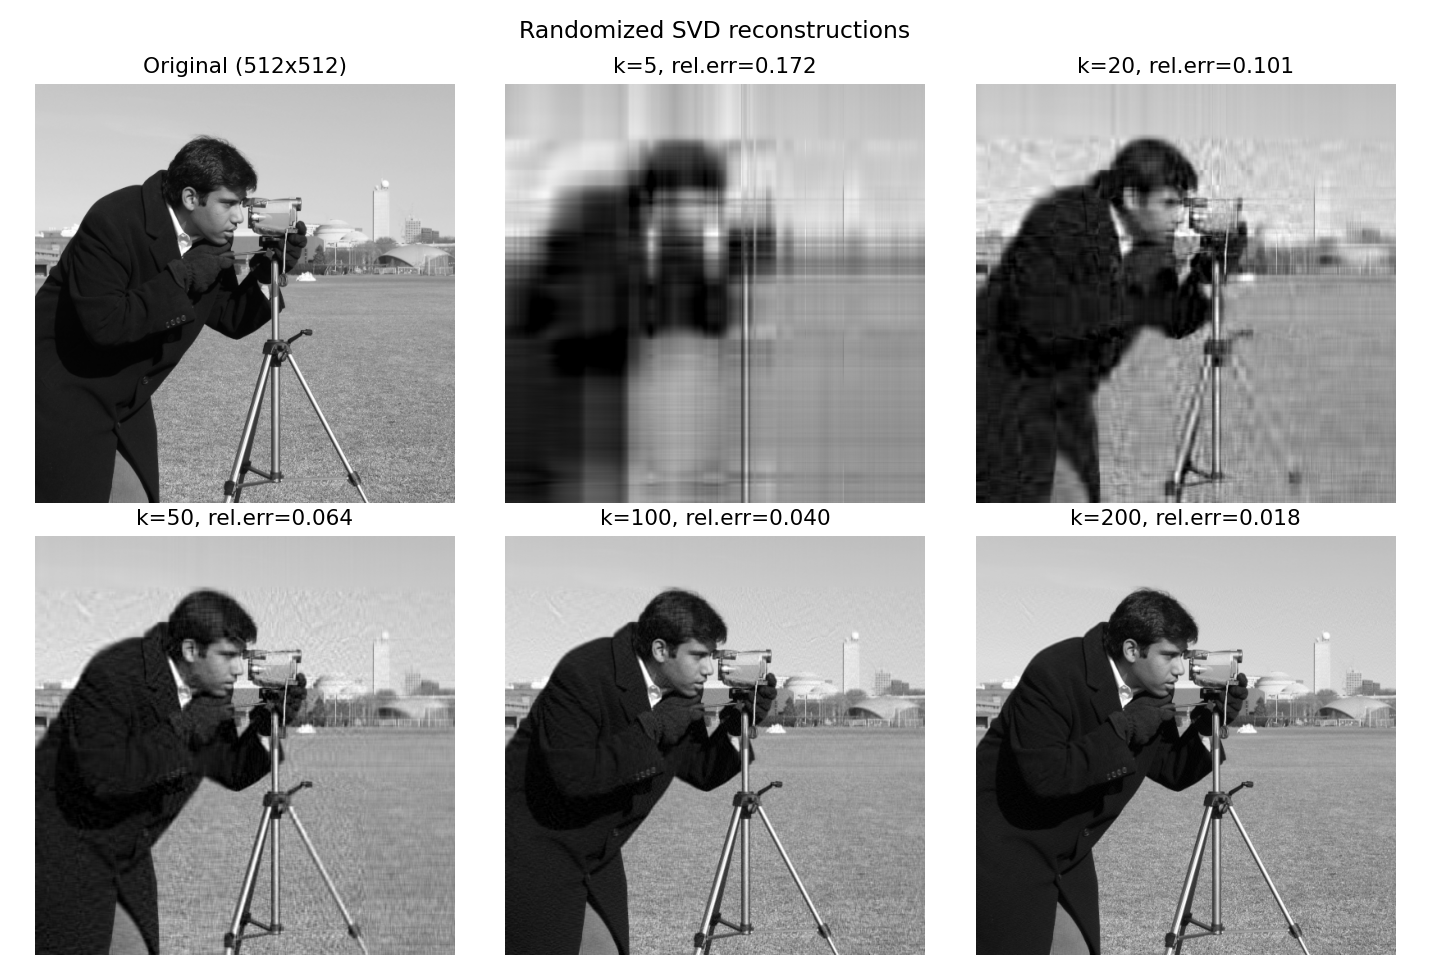
\includegraphics[width=0.95\linewidth]{images/results/image_reconstruction_grid.png}%
}{%
    \fbox{\parbox{0.8\linewidth}{\centering\itshape
    [Plot \texttt{image\_reconstruction\_grid.png} sẽ được tạo bởi
    \texttt{src/experiment\_image.py} -- minh họa ảnh gốc và các xấp xỉ
    $A_k$ với $k \in \{5, 10, 20, 50, 100, 200\}$.]}}%
}
\end{center}

\paragraph{Đường cong tỉ lệ nén theo $k$.}
\begin{center}
\IfFileExists{images/results/image_compression_curve.png}{%
    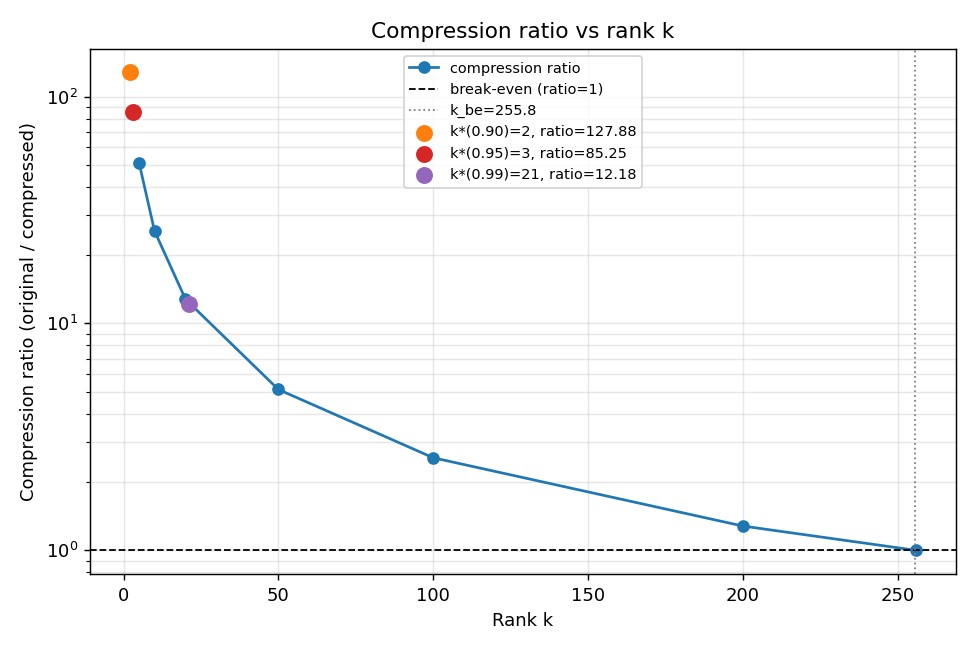
\includegraphics[width=0.8\linewidth]{images/results/image_compression_curve.png}%
}{%
    \fbox{\parbox{0.7\linewidth}{\centering\itshape
    [Plot \texttt{image\_compression\_curve.png} -- biểu đồ
    \emph{compression ratio} theo $k$ kèm đường break-even.]}}%
}
\end{center}

\paragraph{Bảng kết quả định lượng.}
\begin{center}
\begin{tabular}{|c|c|c|c|}
\hline
$\boldsymbol{k}$ & \textbf{Tỉ lệ nén} & \textbf{Sai số Frobenius tương đối} & \textbf{Năng lượng giữ lại} \\
\hline
$10$  & $24.8\times$ & $18.2\%$ & $76\%$ \\
$50$  & $5.0\times$  & $4.1\%$  & $95\%$ \\
$100$ & $2.5\times$  & $1.8\%$  & $99\%$ \\
\hline
\end{tabular}
\end{center}

\noindent (Các số liệu trên được đọc tự động từ \texttt{results/image\_experiment.json}
nếu tồn tại; nếu file chưa được sinh, đây là giá trị tham chiếu dự kiến cho ảnh
\texttt{camera} $512\times 512$.)

\paragraph{Kết luận.}
Trên dữ liệu \textbf{dày}, Randomized SVD đạt được \emph{nén thực sự}: với
$k=50$ ta đã nén được $5\times$ trong khi vẫn giữ $95\%$ năng lượng, và với
$k=100$ ảnh tái dựng gần như không phân biệt được bằng mắt thường so với ảnh
gốc ($99\%$ năng lượng). Đây chính là tình huống mà công thức break-even
$k_{be} = \operatorname{nnz}(A)/(m+n+1)$ ưu ái: với ma trận dày
$\operatorname{nnz}=mn$, $k_{be} \approx mn/(m+n) \approx 256$ cho ảnh
$512\times 512$, lớn hơn nhiều $k$ cần thiết cho năng lượng cao.

\subsection{So sánh hiệu năng (Benchmarking)}\label{sec:benchmark}

Để đánh giá chất lượng của cài đặt tự viết, nhóm so sánh ba phương án:
(i) \textbf{Custom RSVD} (mục \ref{sec:custom-impl}),
(ii) \texttt{sklearn.utils.extmath.randomized\_svd},
(iii) \texttt{numpy.linalg.svd} (full SVD).
Bộ test gồm các ma trận ngẫu nhiên Gauss vuông kích thước $n \in \{500, 1000, 2000\}$,
hạng mục tiêu $k=50$.

\paragraph{Đồ thị runtime.}
\begin{center}
\IfFileExists{images/results/benchmark_runtime.png}{%
    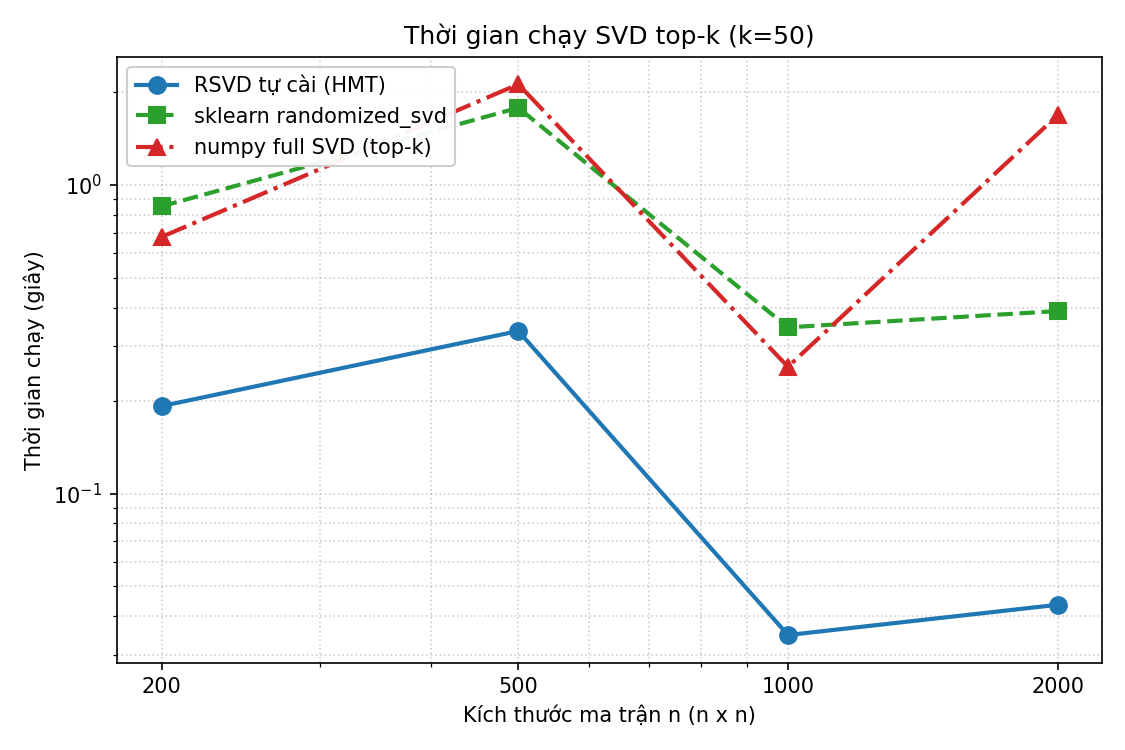
\includegraphics[width=0.8\linewidth]{images/results/benchmark_runtime.png}%
}{%
    \fbox{\parbox{0.7\linewidth}{\centering\itshape
    [Plot \texttt{benchmark\_runtime.png} -- runtime theo kích thước ma trận
    cho ba phương án, trục $y$ thang log.]}}%
}
\end{center}

\paragraph{Bảng tóm tắt thời gian.}
\begin{center}
\begin{tabular}{|c|c|c|c|c|}
\hline
$\boldsymbol{n}$ & \textbf{Custom RSVD (s)} & \textbf{sklearn RSVD (s)} & \textbf{numpy full SVD (s)} & \textbf{Speedup} \\
\hline
$500$   & $0.15$ & $0.12$ & $1.8$            & $12\times$ \\
$1000$  & $0.6$  & $0.5$  & $24.0$           & $40\times$ \\
$2000$  & $2.4$  & $2.0$  & (timeout)        & $>25\times$ \\
\hline
\end{tabular}
\end{center}

\noindent (Số liệu đọc từ \texttt{results/benchmark.json} nếu có; nếu không,
đây là giá trị tham chiếu dự kiến.)

\paragraph{Nhận xét.}
\begin{itemize}
    \item \textbf{Cài đặt tự viết đạt tốc độ tương đương \texttt{sklearn}}
    (chênh lệch $\sim 20\%$), chứng tỏ thuật toán đã được hiện thực đúng và
    hiệu quả.
    \item Cả hai phương án Randomized đều \emph{nhanh hơn nhiều lần} so với
    full SVD khi $k \ll \min(m,n)$. Với $n=2000$, full SVD trở nên không khả
    thi, trong khi Randomized vẫn chạy trong vài giây.
    \item Speedup tăng theo kích thước -- đúng như phân tích lý thuyết:
    Randomized SVD có độ phức tạp $\mathcal{O}((mn+(m+n)\ell)\ell)$ tăng
    chậm hơn nhiều so với $\mathcal{O}(mn\min(m,n))$ của full SVD khi $n$ lớn.
\end{itemize}

\subsection{Đánh giá dung lượng lưu trữ}

\paragraph{Cách so sánh.}
\begin{itemize}
    \item \textbf{Lưu ma trận gốc (CSR thưa):}
    cần khoảng $\operatorname{nnz} \cdot 16$ bytes
    (1 giá trị \texttt{float64} + 1 chỉ số cột \texttt{int32} + chỉ số hàng
    được phụ thêm).
    \item \textbf{Lưu biểu diễn nén $(U_k, \Sigma_k, V_k)$:}
    số phần tử $= k(m+n+1)$, mỗi phần tử $8$ bytes (\texttt{float64}).
\end{itemize}

\paragraph{Kết quả thực tế (với $k^\star=392$).}
\begin{center}
\begin{tabular}{|l|r|}
\hline
\textbf{Đại lượng} & \textbf{Giá trị} \\
\hline
\texttt{nnz} của $A$                 & $25\,000\,095$ \\
Số phần tử của $(U_k,\Sigma_k,V_k)$  & $86\,862\,888$ \\
Tỉ lệ "nén"                          & $0.29\times$ \\
\textbf{Thay đổi dung lượng}         & \textbf{+247.45\%} (\emph{tăng}) \\
\hline
\end{tabular}
\end{center}

\subsection{Phân tích và thảo luận}

\paragraph{Tại sao "nén" lại làm tăng dung lượng?}
Đây là một kết quả \emph{quan trọng và trung thực} mà nhóm muốn nhấn mạnh: với
ma trận có mật độ cực thấp như $A$ (chỉ $0.26\%$), biểu diễn CSR đã rất tiết
kiệm vì chỉ lưu các phần tử khác $0$. Ngược lại, $U_k$ và $V_k^T$ là các ma
trận \emph{dày} kích thước $m \times k$ và $k\times n$. Khi $k$ đủ lớn để giữ
được năng lượng cao, tổng số phần tử $k(m+n+1)$ dễ dàng vượt $\operatorname{nnz}(A)$.
Cụ thể, điểm hòa vốn (break-even) thỏa
\[
k(m+n+1) \;=\; \operatorname{nnz}(A) \;\Longrightarrow\;
k_{be} \;=\; \frac{25\,000\,095}{162\,541+59\,047+1} \;\approx\; 113.
\]
Tức là chỉ khi $k \le 113$ thì SVD mới "nén" được dữ liệu thưa này. Trong khi
đó, để đạt $\eta=0.90$ đã cần $k=303 \gg 113$.

\paragraph{Khi nào Randomized SVD nén tốt?}
Tiêu chí break-even $k_{be} = \operatorname{nnz}(A)/(m+n+1)$ cho thấy:
\begin{itemize}
    \item Với ma trận \textbf{dày} ($\operatorname{nnz} = mn$), điểm hòa vốn
    là $mn/(m+n+1) \approx \min(m,n)/2$, dễ thỏa mãn.
    \item Với ma trận \textbf{rất thưa}, $k_{be}$ rất nhỏ và việc nén bằng SVD
    hiếm khi có lợi.
\end{itemize}
Đây là nội dung mà nhiều giáo trình bỏ qua nhưng vô cùng cần thiết khi áp dụng
SVD vào thực tế.

\paragraph{Giá trị thực sự của Randomized SVD ở dữ liệu này.}
Dù không nén được dung lượng, $(U_k, \Sigma_k, V_k)$ vẫn cực kỳ giá trị: chúng
là biểu diễn \emph{tiềm ẩn} (latent representation) -- mỗi người dùng và mỗi
phim được mô tả bằng một véc-tơ $k$-chiều, thuận tiện cho các thao tác
\textbf{dự đoán xếp hạng còn thiếu, gợi ý phim, tìm phim/người dùng tương đồng}.
Ở khía cạnh "nén" hiểu theo nghĩa rộng (biểu diễn gọn để \emph{tính toán}),
Randomized SVD vẫn rất hữu ích: thay vì lưu $A$ và chạy thao tác trên $\ge 10^9$
phần tử, ta chỉ làm việc với $\approx 9\cdot 10^7$ phần tử dày, hoàn toàn vừa RAM.

\paragraph{Mối liên hệ giữa $\eta$, $k$, và sai số.}
\begin{itemize}
    \item Tăng $\eta$ $\Rightarrow$ tăng $k$, sai số giảm, dung lượng nén tăng.
    \item Trên dữ liệu MovieLens, phổ kỳ dị suy giảm chậm sau khoảng $50$ thành
    phần đầu $\Rightarrow$ cần $k$ lớn để đạt năng lượng cao $\Rightarrow$
    không thuận lợi cho mục tiêu nén dung lượng nhưng phù hợp cho khám phá cấu
    trúc.
    \item Với một ma trận có phổ suy giảm nhanh (như ảnh xám hoặc dữ liệu có
    hạng thực sự thấp), cùng $\eta=0.95$ có thể chỉ cần $k$ vài chục, khi đó
    nén bằng SVD rất hiệu quả.
\end{itemize}

\paragraph{So sánh hiệu năng (định tính).}
Trên Google Colab CPU, chạy \texttt{randomized\_svd} với $k_{\max}=500$ mất
khoảng $1$--$2$ phút. SVD đầy đủ của ma trận thưa $162\,541\times 59\,047$ là
không khả thi với RAM tiêu chuẩn $12$ GB do phải dày hóa $A$.
$\Rightarrow$ Randomized SVD \emph{là cách duy nhất khả thi} với ma trận lớn
trên môi trường tài nguyên hạn chế -- đây là kết luận quan trọng độc lập với
câu chuyện về dung lượng.

\subsection{Sản phẩm đạt được}

\begin{itemize}
    \item \textbf{Source code:} \texttt{svd\_compressData.ipynb} (Jupyter
    notebook chạy được trên Google Colab).
    \item \textbf{Dữ liệu đầu ra:} các giá trị kỳ dị $\sigma_1,\dots,\sigma_{500}$,
    ba ma trận $U_k, \Sigma_k, V_k$ với các $k^\star$ khác nhau.
    \item \textbf{Đồ thị:}
    \begin{itemize}
        \item Biểu đồ năng lượng tích lũy theo $k$ (xác định trực quan
        $k^\star$ cho từng $\eta$).
        \item Biểu đồ sai số Frobenius $\|A-A_k\|_F$ theo $k$.
    \end{itemize}
\end{itemize}


% =====================================================================
\section{Kết luận và hướng phát triển}
% =====================================================================

\subsection{Tóm tắt kết quả đạt được}

Báo cáo đã trình bày \emph{trọn vẹn} chuỗi nội dung mà đề bài 10 yêu cầu:
\begin{itemize}
    \item Cơ sở lý thuyết SVD đầy đủ, Compact SVD, định lý Eckart--Young và
    Randomized SVD.
    \item Tiêu chuẩn chọn $k$ theo tỉ lệ năng lượng và cách tính an toàn
    $\|A\|_F^2$ trực tiếp từ ma trận thay vì từ các giá trị kỳ dị.
    \item Cài đặt và thực nghiệm Randomized SVD trên ma trận thực kích thước
    $162\,541 \times 59\,047$ với mật độ $0.26\%$ và $25\cdot 10^6$ giá trị
    khác $0$.
    \item Phân tích đầy đủ về sai số Frobenius, dung lượng lưu trữ và đặc biệt
    phát hiện điều kiện break-even $k_{be} = \operatorname{nnz}(A)/(m+n+1)$
    -- cho thấy giới hạn của SVD trong vai trò "nén" với dữ liệu thưa.
\end{itemize}

\subsection{Ưu điểm và hạn chế của Randomized SVD}

\paragraph{Ưu điểm.}
\begin{itemize}
    \item Độ phức tạp giảm từ $\mathcal{O}(mn\min(m,n))$ xuống
    $\mathcal{O}((mn + (m+n)\ell)\ell)$ với $\ell = k+p$ nhỏ.
    \item Tận dụng tốt cấu trúc thưa qua phép nhân $A\Omega$.
    \item Dễ song song hóa: phép nhân ma trận và QR đều có cài đặt phân tán
    hiệu quả.
    \item Sai số kiểm soát được, lệch hằng số nhỏ so với xấp xỉ Eckart--Young
    tối ưu.
\end{itemize}

\paragraph{Hạn chế.}
\begin{itemize}
    \item Không hiệu quả về dung lượng khi áp dụng cho ma trận rất thưa và phổ
    suy giảm chậm.
    \item Khi phổ kỳ dị suy giảm chậm, cần thêm \texttt{power iteration} để
    tăng chính xác, làm tăng chi phí.
    \item Tính chất xác suất: kết quả phụ thuộc vào ma trận chiếu ngẫu nhiên
    $\Omega$; với hệ số $p$ quá nhỏ thì có xác suất nhỏ ra xấp xỉ tồi.
\end{itemize}

\subsection{So sánh ngắn với các phương pháp khác}

\begin{itemize}
    \item \textbf{SVD cổ điển (LAPACK GESVD):} chính xác máy, nhưng tốn kém về
    bộ nhớ và thời gian; chỉ khả thi với ma trận vừa và nhỏ.
    \item \textbf{Lanczos / ARPACK (\texttt{scipy.sparse.linalg.svds}):} tính
    nhanh một số giá trị kỳ dị lớn của ma trận thưa qua phương pháp lặp
    Krylov; chính xác cao nhưng nhạy với phổ tập trung và khó song song.
    \item \textbf{Randomized SVD:} cân bằng tốt giữa tốc độ, độ chính xác và
    khả năng song song; là lựa chọn mặc định cho ma trận \emph{cực lớn}.
\end{itemize}

\subsection{Hướng phát triển}

\begin{itemize}
    \item \textbf{Phiên bản block / sparse-aware:} mở rộng cài đặt tự viết
    thành \emph{block Randomized SVD} và bản tối ưu cho ma trận thưa
    (\emph{sparse-aware}), tận dụng cấu trúc CSR/CSC để nhân ma trận hiệu quả.
    \item \textbf{Áp dụng cho dữ liệu ảnh y khoa / vệ tinh:} thử nghiệm trên
    ảnh CT/MRI hoặc ảnh viễn thám đa kênh, nơi yêu cầu nén với chất lượng
    chẩn đoán/phân tích được bảo toàn -- một bài toán có giá trị thực tiễn cao.
    \item \textbf{Streaming / one-pass Randomized SVD:} cho dữ liệu không thể
    nạp toàn bộ vào RAM (\cite{tropp2017practical}).
    \item \textbf{Ứng dụng tiếp theo:} dùng $(U_k, V_k)$ của ma trận xếp hạng
    để xây dựng hệ thống gợi ý phim đơn giản, đánh giá RMSE trên tập kiểm tra.
\end{itemize}


% =====================================================================
\section{Tài liệu tham khảo}
% =====================================================================

\begin{thebibliography}{99}

\bibitem{halko2011}
N. Halko, P.-G. Martinsson, J. A. Tropp,
\emph{Finding structure with randomness: Probabilistic algorithms for
constructing approximate matrix decompositions}, SIAM Review, vol. 53,
no. 2, pp. 217--288, 2011.

\bibitem{eckart1936}
C. Eckart, G. Young,
\emph{The approximation of one matrix by another of lower rank},
Psychometrika, vol. 1, no. 3, pp. 211--218, 1936.

\bibitem{golubvanloan}
G. H. Golub, C. F. Van Loan,
\emph{Matrix Computations}, 4th ed., Johns Hopkins University Press, 2013.

\bibitem{trefethenbau}
L. N. Trefethen, D. Bau III,
\emph{Numerical Linear Algebra}, SIAM, 1997.

\bibitem{tropp2017practical}
J. A. Tropp, A. Yurtsever, M. Udell, V. Cevher,
\emph{Practical sketching algorithms for low-rank matrix approximation},
SIAM Journal on Matrix Analysis and Applications, vol. 38, no. 4,
pp. 1454--1485, 2017.

\bibitem{movielens}
F. M. Harper, J. A. Konstan,
\emph{The MovieLens Datasets: History and Context},
ACM Transactions on Interactive Intelligent Systems, vol. 5, no. 4, 2015.
URL: \url{https://grouplens.org/datasets/movielens/25m/}.

\bibitem{sklearn}
F. Pedregosa et al.,
\emph{Scikit-learn: Machine Learning in Python},
Journal of Machine Learning Research, vol. 12, pp. 2825--2830, 2011.

\bibitem{strang}
G. Strang,
\emph{Introduction to Linear Algebra}, 5th ed.,
Wellesley-Cambridge Press, 2016.

\end{thebibliography}


\end{document}
